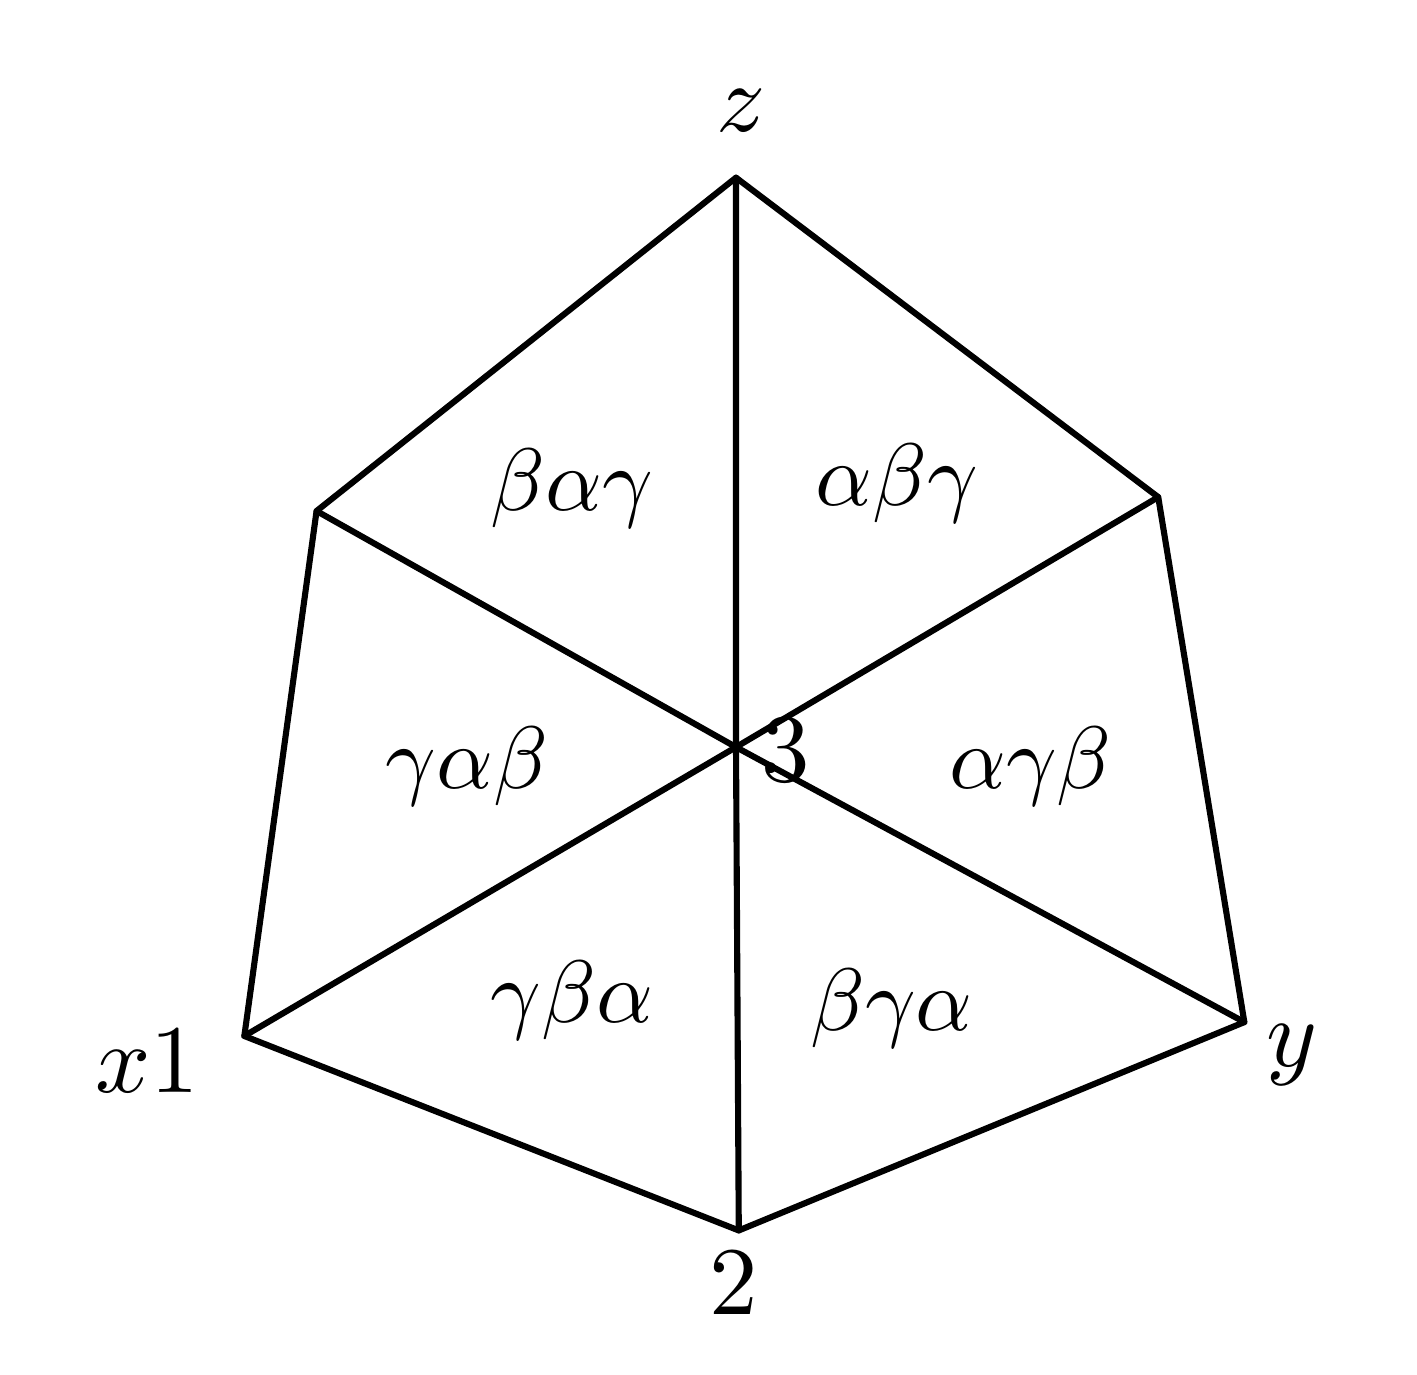
\begin{tikzpicture}[x=1bp,y=-1bp,line cap=round,line join=round]
\path[use as bounding box] (0,0) rectangle (490,475);
\begin{pgfinterruptboundingbox}
\draw[line width=2.2bp] (255,54) -- (407,169) -- (438,358) -- (256,433) -- (78,363) -- (104,174) -- cycle;
\draw[line width=2.2bp] (255,54) -- (255,259) -- (256,433);
\draw[line width=2.2bp] (104,174) -- (255,259) -- (438,358);
\draw[line width=2.2bp] (78,363) -- (255,259) -- (407,169);
\node[inner sep=0pt,outer sep=0pt,anchor=center] at (196,166) {\scalebox{3.2}{\ensuremath{\beta\alpha\gamma}}};
\node[inner sep=0pt,outer sep=0pt,anchor=center] at (313,164) {\scalebox{3.2}{\ensuremath{\alpha\beta\gamma}}};
\node[inner sep=0pt,outer sep=0pt,anchor=center] at (158,266) {\scalebox{3.2}{\ensuremath{\gamma\alpha\beta}}};
\node[inner sep=0pt,outer sep=0pt,anchor=center] at (361,266) {\scalebox{3.2}{\ensuremath{\alpha\gamma\beta}}};
\node[inner sep=0pt,outer sep=0pt,anchor=center] at (196,350) {\scalebox{3.2}{\ensuremath{\gamma\beta\alpha}}};
\node[inner sep=0pt,outer sep=0pt,anchor=center] at (311,353) {\scalebox{3.2}{\ensuremath{\beta\gamma\alpha}}};
\node[inner sep=0pt,outer sep=0pt,anchor=center] at (257,30) {\scalebox{3.5}{\ensuremath{z}}};
\node[inner sep=0pt,outer sep=0pt,anchor=center] at (43,372) {\scalebox{3.5}{\ensuremath{x1}}};
\node[inner sep=0pt,outer sep=0pt,anchor=center] at (455,370) {\scalebox{3.5}{\ensuremath{y}}};
\node[inner sep=0pt,outer sep=0pt,anchor=center] at (254,452) {\scalebox{3.5}{\ensuremath{2}}};
\node[inner sep=0pt,outer sep=0pt,anchor=center] at (273,260) {\scalebox{3.5}{\ensuremath{3}}};
\end{pgfinterruptboundingbox}
\end{tikzpicture}
